%Ohurit komisiu
%Urobili vela prace, Nebolo to lahke

\documentclass[xcolor=dvipsnames]{beamer} 
\usepackage[slovak]{babel}
\usepackage[utf8]{inputenc}
\usepackage{hyperref}
\usecolortheme[named=Plum]{structure} 
\usetheme[height=7mm]{Rochester} 
\setbeamertemplate{items}[ball] 
\setbeamertemplate{blocks}[rounded][shadow=true] 

\useoutertheme{umbcfootline} 

%%%%%%%%%%%%%%%%%%%%%%%%%%%%%%%%%%%%%%%%%%%%%%%%%%%%%%%%%%%%%%%%%%%%%%%%%
%%%%%%%%%%%%%%%%%%%%%%%%%%%%%%%%%%%%%%%%%%%%%%%%%%%%%%%%%%%%%%%%%%%%%%%%%
%Na úvodnej stránke uveďte: meno študenta, názov diplomovej práce a meno vedúceho diplomovej práce.
%Prezentácia by mala trvať asi 12 minút.
%Na stránky uvádzajte malý počet riadkov.
%Vyhýbajte sa používaniu žargónu.
%Používajte starú múdrosť: 1 obrázok je viac než 1000 slov.
%%%%%%%%%%%%%%%%%%%%%%%%%%%%%%%%%%%%%%%%%%%%%%%%%%%%%%%%%%%%%%%%%%%%%%%%%
%%%%%%%%%%%%%%%%%%%%%%%%%%%%%%%%%%%%%%%%%%%%%%%%%%%%%%%%%%%%%%%%%%%%%%%%%

% items enclosed in square brackets are optional; explanation below
\title[GeneRec Analysis]{
ANALYSIS OF THE GENERALIZED \\
RECIRCULATION-BASED LEARNING ALGORITHM \\
IN BIDIRECTIONAL NEURAL NETWORK \\
\vspace{3cm}
DIPLOMA THESIS
}
\author[P. Csiba]{Bc. Peter Csiba \\ Vedúci: doc. Ing. Igor Farkaš, PhD.}
\institute[FMFI UK]{
  UNIVERZITA KOMENSKÉHO V BRATISLAVE\\
  FAKULTA MATEMATIKY, FYZIKY A INFORMATIKY
}
\date{07.07.2013}

\begin{document}

%--- the titlepage frame -------------------------%
\begin{frame}[plain]
  \titlepage
\end{frame}


%%%%%%%%%%%%%%%%%%%%%%%%%%%%%%%%%%%%%%%%%%%%%%%%%%%%%%%%%%%%%%%%%%%%%%%%%
%%%%%%%%%%%%%%%%%%%%%%%%%%%%%%%%%%%%%%%%%%%%%%%%%%%%%%%%%%%%%%%%%%%%%%%%%
%V úvodnej časti prezentujte pojmy a kontext nevyhnutný pre formuláciu úloh riešených v diplomovej práci.
%Na stránky uvádzajte malý počet riadkov.
%Vyhýbajte sa používaniu žargónu.
%Používajte starú múdrosť: 1 obrázok je viac než 1000 slov.
%%%%%%%%%%%%%%%%%%%%%%%%%%%%%%%%%%%%%%%%%%%%%%%%%%%%%%%%%%%%%%%%%%%%%%%%%
%%%%%%%%%%%%%%%%%%%%%%%%%%%%%%%%%%%%%%%%%%%%%%%%%%%%%%%%%%%%%%%%%%%%%%%%%

\begin{frame}{Kontext nevyhnutný pre formuláciu - Neurónové siete}
  %TODO copy some fancy slide explaining NN 
  
  \begin{center} 
    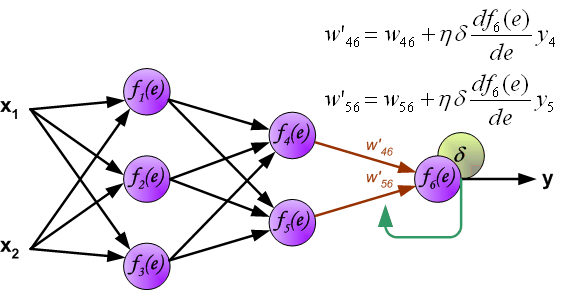
\includegraphics[scale=0.5]{img/bp.png}
  \end{center} 
  \begin{center} 
    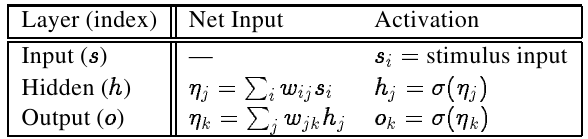
\includegraphics[scale=0.5]{img/table_bp.png}
  \end{center} 
\end{frame}

\begin{frame}{Kontext nevyhnutný pre formuláciu - GeneRec}
  \begin{itemize} 
    \item Biologically plausible error-driven learning using local activation differences: The generalized recirculation algorithm (O'Reilly 1996).
  \end{itemize} 
  
  \begin{center} 
    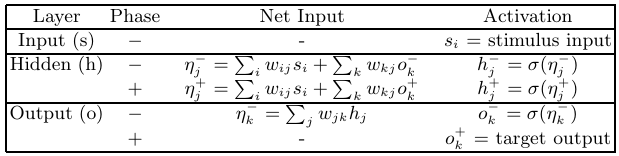
\includegraphics[scale=0.5]{img/generec_activations.png}
  \end{center} 
\end{frame}


%Bidirectional Activation-based Learning algorithm (BAL) shares with GeneRec
%the phase-based activations and unit types, but differs from it by the connectivity
%that allows completely bidirectional associations to be established (GeneRec
%focuses on input-to-output mapping). Unlike GeneRec, BAL uses two pairs of
%weight matrices for each activation phase. In addition, in BAL we do not use
%dynamical settling process but compute the activations in one step as described
%in Table 2.
\begin{frame}{Kontext nevyhnutný pre formuláciu - BAL}
  \begin{itemize}
    \item BAL := Bidirectional Activation-based Neural Network Learning Algorithm (Farkaš and Rebrová, 2013).
    %TODO 
  \end{itemize}
  
  \begin{center}
    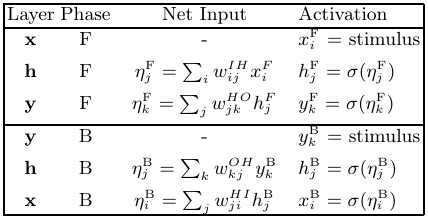
\includegraphics[scale=0.5]{img/bal_activations.png}
  \end{center}  
\end{frame}


%%%%%%%%%%%%%%%%%%%%%%%%%%%%%%%%%%%%%%%%%%%%%%%%%%%%%%%%%%%%%%%%%%%%%%%%%
%%%%%%%%%%%%%%%%%%%%%%%%%%%%%%%%%%%%%%%%%%%%%%%%%%%%%%%%%%%%%%%%%%%%%%%%%
%V nadväznosti na úvodnú časť formulujte cieľ diplomovej práce.
%Na stránky uvádzajte malý počet riadkov.
%Vyhýbajte sa používaniu žargónu.
%Používajte starú múdrosť: 1 obrázok je viac než 1000 slov.
%%%%%%%%%%%%%%%%%%%%%%%%%%%%%%%%%%%%%%%%%%%%%%%%%%%%%%%%%%%%%%%%%%%%%%%%%
%%%%%%%%%%%%%%%%%%%%%%%%%%%%%%%%%%%%%%%%%%%%%%%%%%%%%%%%%%%%%%%%%%%%%%%%%

\begin{frame}{Cieľ diplomovej práce} 
  \begin{enumerate} 
%    \item Study the literature on general recirculation-based learning algorithms in
%    neural networks and write the state-of-the art of the topic (including deep
%    learning).
    \item Implement the GeneRec learning algorithm and test its properties using
    selected data sets.
    \item Consider suitable modifications of the algorithm aimed at improving the
    network performance.
    \item Analyse the convergence of the BAL network aimed at finding parameters on which the convergence depends. 
  \end{enumerate} 
  
  \begin{center}
    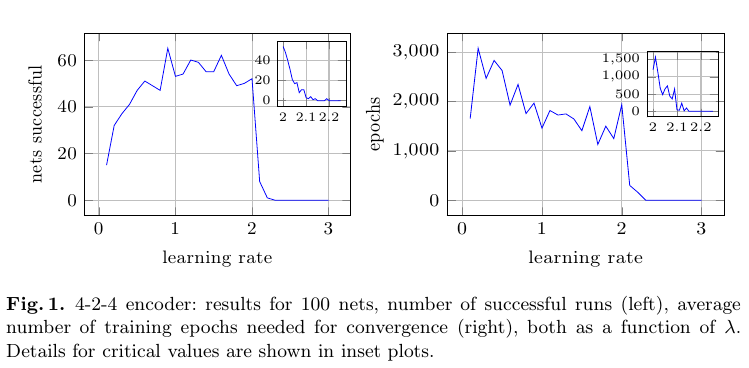
\includegraphics[scale=0.40]{img/bal_performance.png}
  \end{center}  
  
\end{frame} 

%%%%%%%%%%%%%%%%%%%%%%%%%%%%%%%%%%%%%%%%%%%%%%%%%%%%%%%%%%%%%%%%%%%%%%%%%
%%%%%%%%%%%%%%%%%%%%%%%%%%%%%%%%%%%%%%%%%%%%%%%%%%%%%%%%%%%%%%%%%%%%%%%%%
%V ďalšej časti prezentujte vlastný prínos a vlastné výsledky porovnajte s výsledkami iných. Charakterizujte použité metódy.
%Na stránky uvádzajte malý počet riadkov.
%Vyhýbajte sa používaniu žargónu.
%Používajte starú múdrosť: 1 obrázok je viac než 1000 slov.
%%%%%%%%%%%%%%%%%%%%%%%%%%%%%%%%%%%%%%%%%%%%%%%%%%%%%%%%%%%%%%%%%%%%%%%%%
%%%%%%%%%%%%%%%%%%%%%%%%%%%%%%%%%%%%%%%%%%%%%%%%%%%%%%%%%%%%%%%%%%%%%%%%%

\begin{frame}{Vlastný prínos a vlastné výsledky}
  \begin{itemize}
    \item Zrekonštruovanie výsledkov GeneRec a BAL. 
    \item Analýza mňou navrhnutých atribútov siete BAL v priebehu učenia. 
    \item Dôkaz zvýšenia úspešnosti pri výbere sietí so vzdialenejšími skrytými reprezentáciami. 
  \end{itemize} 
  
  \begin{center}
    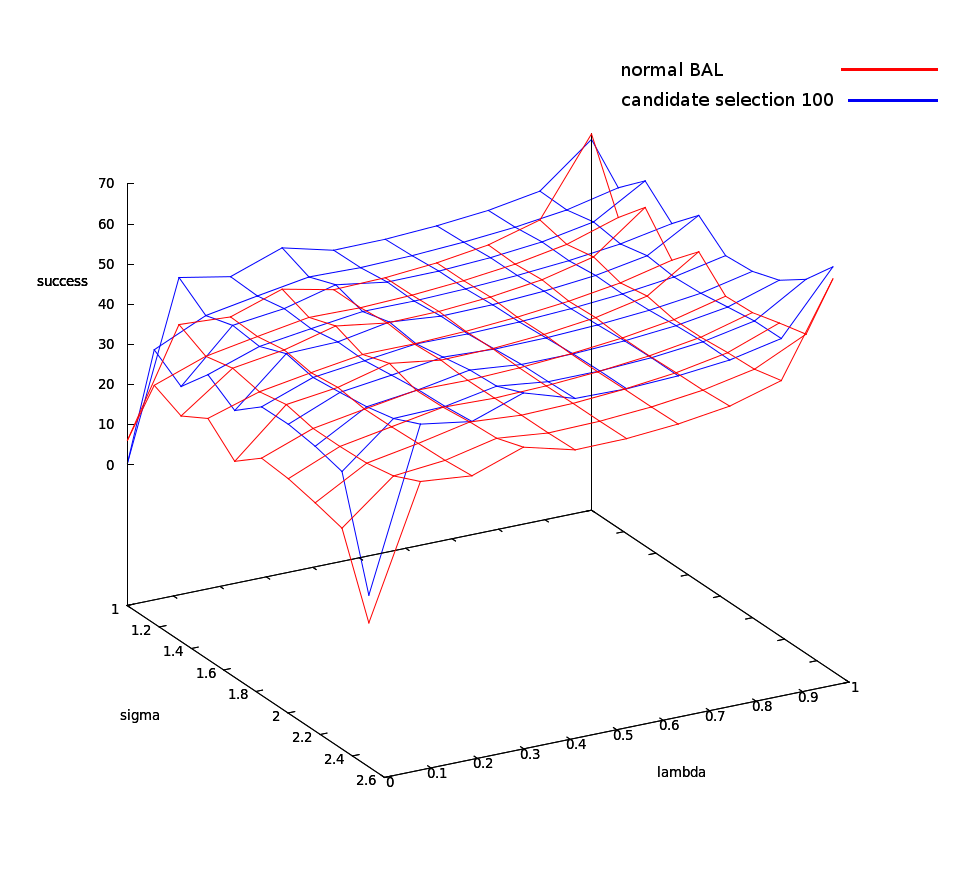
\includegraphics[scale=0.20]{img/compare_normal_and_hdist2.png}
  \end{center} 
\end{frame}

\begin{frame}{Porovnanie s výsledkami iných}
  \begin{center}
    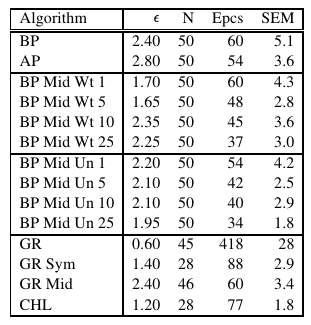
\includegraphics[scale=0.5]{img/comparison.png} 
    \begin{tabular}{|l|l|l|l|}
      \hline
      Algorithm&epsilon&N=10000&Epcs\\
      \hline
      BAL orig &0.9&65/100&2000\\
      \hline
      BAL&0.7&5885&10000\\
      \hline
      BAL candidate&0.7&7024&30000\\
      \hline
      BAL long run&0.7&7934&500000\\
      \hline
    \end{tabular}\\

{\tiny Results for the 4-2-4 encoder problem. $\epsilon$ is the optimal learning rate, $N$ is the number of networks that successfully solved the problem (out of 50), $Epcs$ is the mean number of epochs required to reach criterion, and $SEM$ is the standard error of this mean.} 
  \end{center} 
\end{frame}

\begin{frame}{Charakterizujte použité metódy - čo nefungovalo}
  \begin{itemize}
    \item Doteraz sme vyskúšali viacero modifikácií: 
    \begin{itemize} 
      \item Momentum učenia.
      \item Batch update váh. 
      \item Shuffle vstupov. 
      \item Cielené generovanie počiatočných váh. 
      \item Dropout - vynechanie niektorých skrytých neurónov. 
      \item Iné učiace pravidlá, napr. CHL symetric learning rule.
    \end{itemize} 
    \item V prípade 4-2-4 encoder-a sme dosiahli 70-75\% úspešnosť, pričom Backpropagation má 100\% úspešnosť. 
  \end{itemize} 
\end{frame} 

\begin{frame}{Charakterizujte použité metódy - Zobrazenie priebehu - Good}
    \begin{center}
      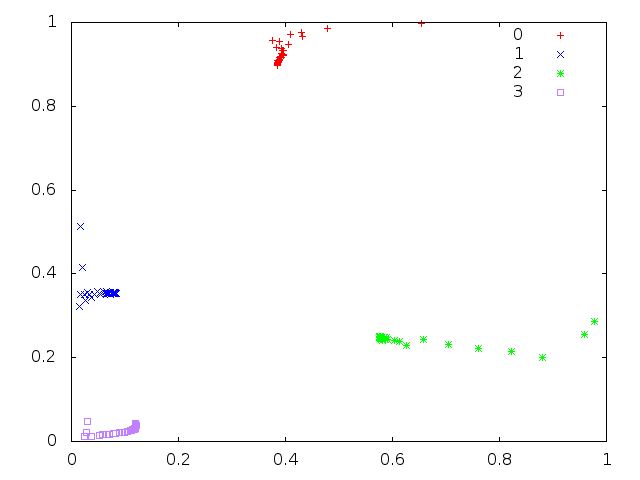
\includegraphics[scale=0.5]{img/nice.png}
    \end{center} 
\end{frame} 
\begin{frame}{Charakterizujte použité metódy - Zobrazenie priebehu - Good}
    \begin{center}
      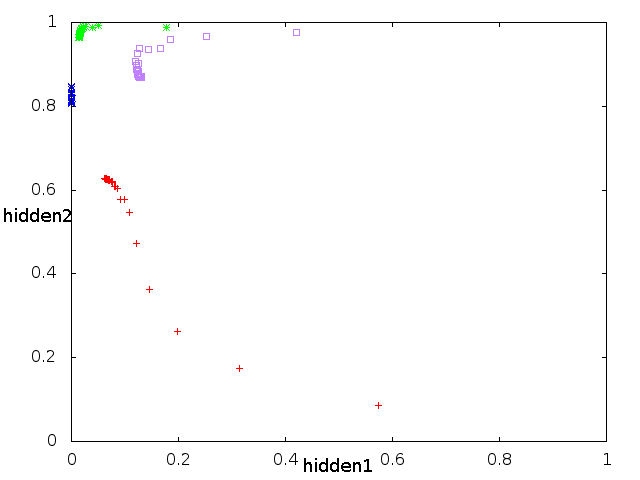
\includegraphics[scale=0.5]{img/left_top.png}
    \end{center} 
\end{frame}

    
\begin{frame}{Charakterizujte použité metódy - Zobrazenie priebehu - Bad}
    \begin{center}
      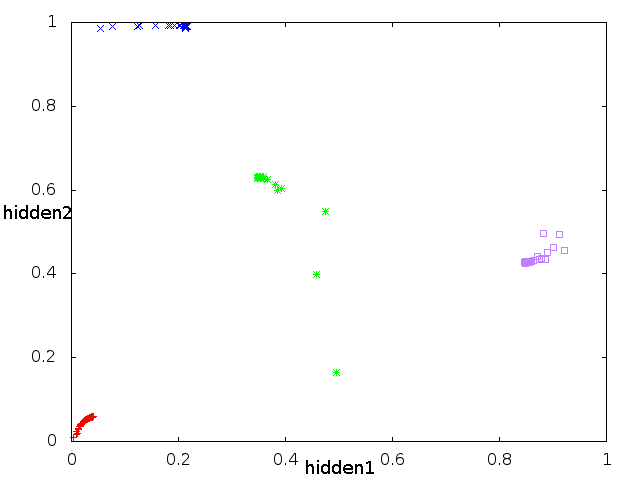
\includegraphics[scale=0.5]{img/tazisko.png}
    \end{center} 
\end{frame}
\begin{frame}{Charakterizujte použité metódy - Zobrazenie priebehu - Bad}
    \begin{center}
      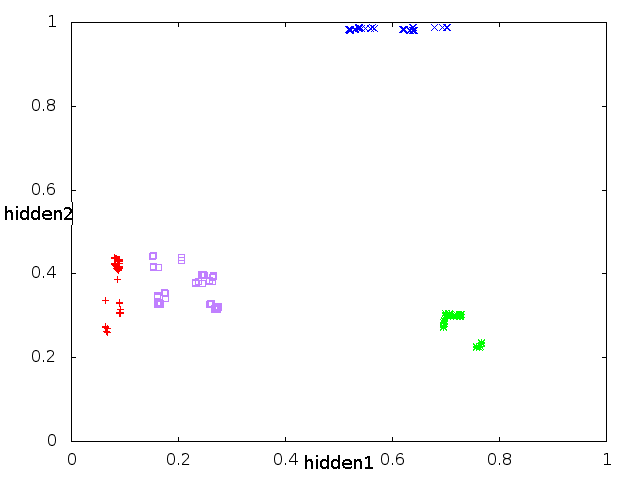
\includegraphics[scale=0.5]{img/non-convergent.png}
    \end{center} 
\end{frame}


%%%%%%%%%%%%%%%%%%%%%%%%%%%%%%%%%%%%%%%%%%%%%%%%%%%%%%%%%%%%%%%%%%%%%%%%%
%%%%%%%%%%%%%%%%%%%%%%%%%%%%%%%%%%%%%%%%%%%%%%%%%%%%%%%%%%%%%%%%%%%%%%%%%
%Na záver sformulujte možnosti ďalšieho rozpracovania práce.
%Na stránky uvádzajte malý počet riadkov.
%Vyhýbajte sa používaniu žargónu.
%Používajte starú múdrosť: 1 obrázok je viac než 1000 slov.
%%%%%%%%%%%%%%%%%%%%%%%%%%%%%%%%%%%%%%%%%%%%%%%%%%%%%%%%%%%%%%%%%%%%%%%%%
%%%%%%%%%%%%%%%%%%%%%%%%%%%%%%%%%%%%%%%%%%%%%%%%%%%%%%%%%%%%%%%%%%%%%%%%%

\begin{frame}{Možnosti ďalšieho rozpracovania práce - nad čím uvažujeme}
  \begin{itemize} 
    \item Matematická formulácia aproximácie dynamického systému BAL a skúmanie jeho konvergencie. 
    \item Učenie ako hľadanie stacionárneho bodu dynamického systému.
    \item Urýchlenie konvergencie pomocou momentumu. 
  \end{itemize} 
\end{frame} 

\begin{frame}{Priestor na otázky}
  \begin{center}
  
\includegraphics[scale=0.75]{img/question.png}
  \end{center}
%  Aktuálna verzia: \url{https://github.com/Petrzlen/diplomovka}
\end{frame}

\begin{frame}{Ďakujem za pozornosť!}
  \begin{center}
{\bf Ďakujem za pozornosť!} 
  \end{center}
  
  \vspace{3cm}
  
  \begin{center}
  \small{P.S. Ospravedlňujeme sa za kvalitu obrázkov.}
  \end{center}
\end{frame}

\end{document}

